\documentclass[a4paper]{article}

\usepackage[paper=a4paper, left=1.5cm, right=1.5cm, bottom=1.5cm, top=3.5cm]{geometry}
\usepackage[spanish,activeacute]{babel}
\usepackage{amsthm}
\usepackage{amsmath}
\usepackage{amsfonts}
\usepackage{amssymb}
\usepackage{alltt}
\usepackage{graphicx} %Para incluir el logo de la UBA
\usepackage{caratula} %Para armar el cuadro de integrantes
\usepackage{multirow} %Para poder poner varias lineas juntas sin divisiones en una tabla
\usepackage[lined,ruled,linesnumbered]{algorithm2e}
\usepackage{url}
%\usepackage{algorithmic}
\usepackage{algpseudocode}
\usepackage{scrextend}
\usepackage{blindtext}
\usepackage{float}
\usepackage[utf8]{inputenc}

%Cosas para escribir codigo fuente
%Fuente: http://en.wikibooks.org/wiki/LaTeX/Source_Code_Listings
\usepackage{listings}
\usepackage{color}

\setcounter{secnumdepth}{5}

\definecolor{mygreen}{rgb}{0,0.6,0}
\definecolor{mygray}{rgb}{0.5,0.5,0.5}
\definecolor{myorange}{rgb}{1,0.4,0.2}
\definecolor{myblue}{rgb}{0,0,0.65}

%Configuracion para los listings
\lstset{ %
  backgroundcolor=\color{white},   % choose the background color; you must add \usepackage{color} or \usepackage{xcolor}
  basicstyle=\small,        % the size of the fonts that are used for the code
  breakatwhitespace=false,         % sets if automatic breaks should only happen at whitespace
  breaklines=true,                 % sets automatic line breaking
  captionpos=b,                    % sets the caption-position to bottom
  commentstyle=\color{mygreen},    % comment style
  deletekeywords={...},            % if you want to delete keywords from the given language
  escapeinside={\%*}{*)},          % if you want to add LaTeX within your code
  extendedchars=true,              % lets you use non-ASCII characters; for 8-bits encodings only, does not work with UTF-8
  frame=single,                    % adds a frame around the code
  keywordstyle=\color{myblue},       % keyword style
  language=Octave,                 % the language of the code
  morekeywords={*,...},            % if you want to add more keywords to the set
  numbers=left,                    % where to put the line-numbers; possible values are (none, left, right)
  numbersep=5pt,                   % how far the line-numbers are from the code
  numberstyle=\tiny\color{mygray}, % the style that is used for the line-numbers
  rulecolor=\color{black},         % if not set, the frame-color may be changed on line-breaks within not-black text (e.g. comments (green here))
  showspaces=false,                % show spaces everywhere adding particular underscores; it overrides 'showstringspaces'
  showstringspaces=false,          % underline spaces within strings only
  showtabs=false,                  % show tabs within strings adding particular underscores
  stepnumber=1,                    % the step between two line-numbers. If it's 1, each line will be numbered
  stringstyle=\color{myorange},     % string literal style
  tabsize=2,                       % sets default tabsize to 2 spaces
  title=\lstname                   % show the filename of files included with \lstinputlisting; also try caption instead of title
}

\renewcommand{\lstlistingname}{C\'{o}digo}

\lstset{language=C++,caption={Descriptive Caption Text},label=DescriptiveLabel}


%\topmargin = -1cm
%\textheight = 24cm 

\begin{document}

\integrante{Rodriguez, Pedro}{xxx/12}{}
\integrante{Vargas Telles, Matías}{318/12}{}


\def\Materia{Algoritmos y Estructuras de Datos III}
\def\Titulo{Trabajo Pr\'{a}ctico 1}
\def\Fecha{FECHA XXXXXXXXXXXXXXXXXXXXXXX}

%----- CARATULA -----%

\thispagestyle{empty}

\begin{center}
	
\includegraphics[scale = 0.25]{logo_uba.jpg}
\end{center}

\vspace{5mm}

\begin{center}
	{\textbf{\large UNIVERSIDAD DE BUENOS AIRES}}\\[1.5em]
	{\textbf{\large Departamento de Computaci\'{o}n}}\\[1.5em]
    {\textbf{\large Facultad de Ciencias Exactas y Naturales}}\\
    \vspace{35mm}
    {\LARGE\textbf{\Materia}}\\[1em]    
    \vspace{15mm}
    {\Large \textbf{\Titulo}}\\[1em]
    \vspace{15mm}
    {\textbf{\Large \Fecha}}\\
    \vspace{15mm}
    \textbf{\tablaints}
\end{center}

\newtheorem{teo}{Teorema}[section]
\newtheorem{propo}{Proposici\'{o}n}[section]
\newtheorem{lema}{Lema}[section]
\newtheorem{coro}{Corolario}[section]
\newtheorem{defi}{Definici\'{o}n}[section]

\newpage
\thispagestyle{empty}
\tableofcontents

\parskip=5pt
\setlength{\parindent}{0pt}

\newpage
\setcounter{page}{1}
\pagenumbering{arabic}
\pagestyle{plain}

\newpage


\newcommand{\Asig}{\ensuremath{\leftarrow}}	
\newcommand{\AndY}{\ensuremath{\wedge}}
\newcommand{\Or}{\ensuremath{\vee}}
\newcommand{\Not}{\ensuremath{\neg}}
\newcommand{\NotEq}{\ensuremath{\neq}}
\newcommand{\MayorIg}{\ensuremath{\geq}}
\newcommand{\tabu}{\hspace*{0.7cm}}
\newcommand{\ctabu}{\hspace*{0.8cm}}
\newcommand{\htabu}{\hspace*{0.35cm}}
\newcommand{\moduloNombre}[1]{\textbf{#1}}




% AGREGAR LA CARATULA (Y UNA INTRODUCCION?)

\section{Cambios realizados con respecto a la primera entrega}
\subsection{Problema 1}
Se agregó el informe\\
Se modificó ligeramente el código para evitar analizar casos repetidos o innecesarios.
\subsection{Problema 2}
 Se agregó el informe\\
Se modificó el código para no realizar un cociente haciendo un producto en su lugar para ordenar los elementos.
\subsection{Problema 3}
Se agregó el informe
\section{Problema 1 - Puente sobre lava caliente}
\index{Problema 1 - Puente sobre lava caliente}



\subsection{Descripci\'on del problema a resolver}

Este problema nos plantea una situación en la cual un individuo desea atravesar un puente. Este puente está compuesto de una cantidad $n$ de tablones que pueden estar rotos o sanos. A su vez nuestro personaje puede saltar hasta una cantidad de $c$ de tablones por salto. Nuestro objetivo entonces es brindar una secuencia de saltos posibles que sea mínima en cantidad de saltos y que garanticen la integridad física del individuo impidiendo que pise tablones rotos.


Veamos algunos ejemplos para comprender mejor este enunciado:  

Instancia 1:

\begin{figure}[H]
\centering

\includegraphics[scale=0.5]{ej1/tabl_1.png}
\end{figure}

En este caso la representación de la instancia que recibiremos como entrada será:

\begin{addmargin}[4em]{0em}
\textsf{8 2 0 0 1 0 0 1 0 0} \\
\textsf{0}
\end{addmargin}

En donde 8 es la cantidad total ($n$) de tablones, 2 ($c$) el salto máximo medido en tablones. Luego $n$ ceros o unos tales que $1$ representa un tablón roto y $0$ el estado contrario. El 0 final indica que termina la instancia.

La solución a esta instancia consta de 4 saltos. El primero al tablón 2, luego al 5, luego al 8 y finalmente fuera del puente. Esta solución la devolveremos de acuerdo al formato solicitado de la siguiente manera:

\begin{addmargin}[4em]{0em}
\textsf{4 2 5 8 11} \\
\end{addmargin}

Notemos 2 aspectos relevantes a la interpretación del problema en esta solución. En primer lugar, la cantidad $c$ de tablones máxima que se puede saltar implica que no puede haber más de $c$ tablones entre el tablón del cual se parte y el tablón al que se llega. De esta manera, por ejemplo, partiendo del tablón 2 con $c=2$ se podra llegar como máximo al tablón 5. 
Otro detalle importante consiste en notar que se empieza fuera del puente y se debe terminar fuera de él también. Podria verse como que existe un tablón $0$ del cual se parte y cualquier número mayor a $n$ en la salida indica que estamos fuera del tablón. Por este motivo, en este caso, el último valor de la salida es 11, que corresponde a realizar el salto máximo desde el tablón 1. 

Dicho esto veamos que para este caso sólo había una solución posible que minimiza los saltos y también que en cada salto el personaje saltarin termina en el tablón sano más lejano posible. Más adelante en este informe demostraremos que esta intuición efectivamente sirve para garantizar los mínimos saltos posibles, sin embargo, consideramos importante notarlo en estas instancias previas.

Analicemos otra instancia:

\begin{figure}[H]
\centering

\includegraphics[scale=0.5]{ej1/tabl_3.png}
\end{figure}

En este caso la entrada recibida se verá asi: 

\begin{addmargin}[4em]{0em}
\textsf{8 3 0 0 1 0 0 0 0 0} \\
\textsf{0}
\end{addmargin}

Nuevamente tenemos 8 tablones pero ahora solo uno roto y podemos saltar de a 3. 

Veamos también la salida de nuestro algoritmo:

\begin{addmargin}[4em]{0em}
\textsf{3 4 8 12} \\
\end{addmargin}

Lo destacable de esta instancia es que permite varias soluciones. Si bien, como explicamos previamente, nuestro algoritmo siempre salta al tablón sano más lejano, una solución posible consite en saltar primero al tablón 4, luego al 7 y luego salir del puente, sin saltar más veces. Cualquier solución de saltos mínimos es permitida como salida de este problema.

Por último notemos la siguiente instancia

\begin{figure}[H]
\centering

\includegraphics[scale=0.5]{ej1/tabl_2.png}
\end{figure}

Cuya entrada es: 
\begin{addmargin}[4em]{0em}
\textsf{8 3 0 0 1 1 1 1 0 0} \\
\textsf{0}
\end{addmargin}

La salida en este caso es:

\begin{addmargin}[4em]{0em}
\textsf{no} \\
\end{addmargin}

Este \textbf{no} indica que no hay solución para esta instancia, dato que puede obtenerse de la observación de la entrada, ya que tenemos más tablones rotos consecutivos de los que podemos saltar en un salto.

Habiendo recorrido entonces un espectro amplio de casos posibles, en la siguiente sección describiremos más detalladamente las ideas involucradas(con su demostración) en la solución de este problema.

\subsection{Ideas desarrolladas para la resoluci\'on}

Como ya hemos expresado previamente, hay una premisa que pareciera guiarnos hacia la solución de este problema y es la idea de que, para minimizar la cantidad de saltos involucrados en el cruce del puente, en cada salto el personaje debe dirigirse hacia el tablón sano más lejano. 

Veamos en la figura siguiente cómo procedera nuestro algoritmo para una instancia particular de 8 tablones y salto máximo 2 tablones:

\begin{figure}[H]
\centering
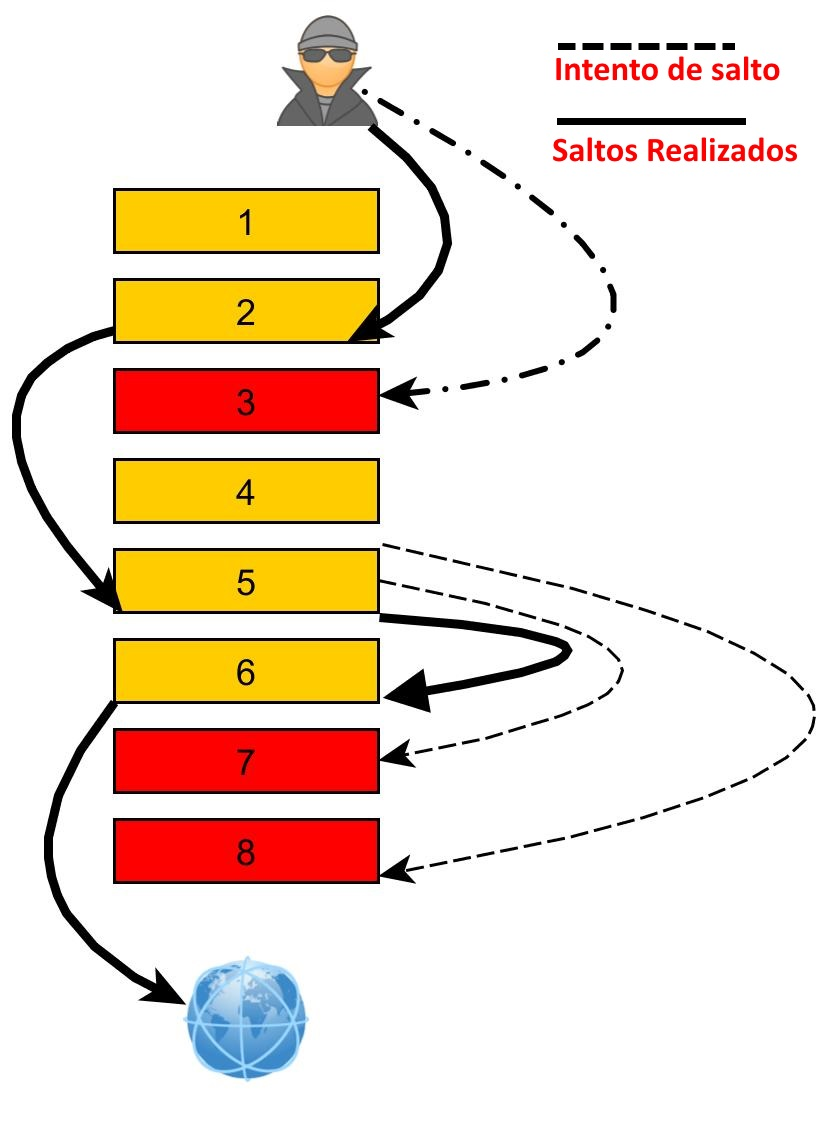
\includegraphics[scale=0.32]{ej1/unnamed0.jpg}
\end{figure}

Se ve claramente cómo cada vez que llega a un tablón prueba el tablón más lejano a su alcance, retrocediendo en caso de encontrar un tablón roto. 

En la siguiente sección formalizaremos esta idea y probaremos qué efectivamente los saltos mínimos se consiguen optando golosamente por el salto más lejano en cada momento.


\subsection{Justificaci\'on de correctitud}

A continuaci\'on presentamos un pseudoc\'odigo del algoritmo goloso empleado a fin de demostrar su correctitud.

\begin{algorithm}[H]
	 cantSaltos $\leftarrow$ 0 \\
     \While{no salí del puente}{
    	salto C tablones\\
        cantSaltos + 1 \\
        \While{no estoy en un tablón sano}{
        	retrocedoUno\\
            \If{volvíAlPrincipio}{no es posible cruzar\\}
         registroDóndeEstoy \\
         }
         }
         \caption{Pseudoc\'odigo para demostrar correctitud.Se asume que se recibe el puente con su cantidad de tablones y el salto máximo permitido}
\end{algorithm}

Este pseudocódigo no es más que una transcipción de la idea original en donde en cada iteración del ciclo principal se avanzan c tablones, se aumentan los saltos necesarios y si el tablón esta roto se retrocede o bien hasta encontrar un tablón sano o bien hasta volver al origen del salto en cuyo caso no habrá solución. Demostraremos entonces que este procedimiento efectivamente cumple con lo pedido.

Supongamos que \textbf{el problema tiene soluci\'on}, que \textbf{estamos en el tabl\'on $k$}, y queremos decidir a cu\'al de los tablones en el intervalo $(k..k+C+1]$ saltar para minimizar la cantidad de pasos en la que voy a cruzar el puente. 

Entonces, como la cantidad de tablones es finita y s\'olo \textbf{avanzamos hacia adelante}, deber\'ia haber \textbf{un tabl\'on \'optimo }que permita \textbf{minimizar la cantidad de saltos totales}.

Supongamos que decido saltar al tabl\'on $k+j_{1}$ pudiendo haber saltado al tabl\'on $k+j_{2}$, con $j_{1} < j_{2} \leq C$. En el siguiente paso, tambi\'en voy a querer saltar al tabl\'on que minimize la cantidad total de saltos que voy a dar desde $k+j_{1}$. Como asumimos que el problema tiene soluci\'on, \textbf{este tabl\'on seguro que existe}. Llam\'emoslo $t$, donde $t > k+C$ (pues de lo contario ya habr\'ia llegado a este tabl\'on en el paso anterior). 

Observemos entonces que este tabl\'on si es accesible desde el tabl\'on $k+j_{1}$ entonces tambi\'en lo es desde el tabl\'on $k+j_{2}$ pues $j_{1} < j_{2} $ pero, la rec\'iproca no vale siempre pues podr\'ia suceder que este tabl\'on $t$ cumpla que $k+j_{1}+C+1 < t \leq k+j_{2}+C+1 $ (i.e. no podr\'ia llegar a $t$ desde $k+j_{1}$ mientras que s\'i podr\'ia haberlo alcanzado si hubiera saltado a $k+j_{2}$). 

De esta manera, saltando siempre al tablón sano más lejano Luego, nuestro algoritmo cumple el invariante de que en cada paso, saltamos a un tabl\'on perteneciente al conjunto de tablones \'optimo (es decir, que minimiza la cantidad de pasos totales). 

Si el problema no tuviera soluci\'on, entonces seguro es porque hay alguna secuencia de tablones malos de longitud mayor o igual que C. Este caso lo contemplamos en el pseudoc\'odigo de m\'as arriba: si en alg\'un momento el sujeto salta los C tablones y despues retrocede esos mismos C tablones, entonces asumimos que el problema no tiene soluci\'on y finalizamos.

\subsection{Justificaci\'on cota de complejidad}

Adicionalmente a la resolución del problema, se nos solicitó que nuestro algoritmo se comportara linealmente en el tiempo respecto de la cantidad ($n$) de tablones del puente recibido como entrada (i.e. complejidad  $O(n)$ ). 

Como ya dijimos en secciones anteriores, el algoritmo hace que el individuo intente saltar la mayor cantidad de tablones posibles en funci\'on de su capacidad $c$ de salto y, si al intentar saltar esa cantidad de tablones se diera cuenta que va a caer en uno de los tablones rotos, el individuo deber\'ia ir retrocediendo uno a uno en los tablones anteriores al que pretend\'ia llegar hasta encontrar uno que no este roto, y saltar a ese. \\

Para mostrar que no hace falta más de $n$ iteraciones para recorrer el puente, vamos a mostrar que cada 2 iteraciones se avanzan al menos $c$ casilleros si hay solución (realizando $c$ veces el ciclo de retroceso) y que, entonces, la guarda del ciclo principal se reduce en $c$ cada 2 iteraciones. 

De esta manera, en cada iteración del ciclo principal, por cada vez que se ejecuta el subciclo de retroceso (tiempo constante $O(1)$), se descuenta una iteración de la guarda del ciclo principal, pudiendo decirse entonces que el algoritmo toma tiempo lineal (en la cantidad de tablones). 

Veamos que en la \textbf{iteración $i$}si el sujeto \textbf{estaba en el tabl\'on $k$} es porque \textbf{retrocedió $j$ tablones en el paso $i-1$}( $j<c$, ya que si $j=c$ entonces no hay solución); entre el tabl\'on $k$ y el $k+j$ no hay ning\'un tabl\'on sano. De esta forma, en el paso $i+1$ el sujeto tendr\'a que retroceder no m\'as de $k+c-k-j = c-j$ tablones luego de saltar, ya que los $j$ tablones después de k no están sanos. 

Esto implica que entre el paso $i-1$ y el paso $i$, en el peor caso el sujeto no recorreria m\'as de $c-j+j=c$ tablones, habiendo avanzado un total de $c-j+k+j+1-k-1 = c$ tablones.

As\'i vemos entonces que se cumple que en el peor caso cada 2 iteraciones se avanzan $c$ tablones que son descontados de la guarda del ciclo principal. De esta forma, como dicho ciclo contiene asignaciones de tiempo constante y el subciclo de retroceso también, el recorrido que hace el algoritmo es lineal ya que las iteraciones constantes que realiza en el subciclo, las descuenta del ciclo más grande.

\begin{lstlisting}[caption=Fragmento de código c++ encargado del ciclo principal y el subciclo de retroceso]
	  actual = 0; cantPasos = 0;	

	  while(actual <= n) {			// hasta haber cruzado el puente, hago..
		
			temp = 0; actual += c; // asinaciones O(1)
		
			while(temp < c && puente[actual] == 1) {	// retrocedo lo necesario	
														
			    actual--; //descuento iteraciones del ciclo grande O(1)
			    temp++;
		    }
		    if(temp == c) {cout << "no" << endl; break; }	// sin solucion. No analizamos complejidad de I/O
		
	        res[cantPasos] = actual; cantPasos++;			// registro el nuevo salto
	  }
\end{lstlisting}


\subsection{Testeos de complejidad}
En la presente sección analizaremos experimentalmente la complejidad temporal del algoritmo propuesto para la resolución del problema planteado.

\subsubsection{Medición de tiempos y generación de entradas}
Para medir los tiempos usamos la biblioteca \textit{time.h}. Medimos solamente nuestra implementación (el tiempo empleado por el ciclo principal) sin contar las operaciones de entrada/salida.  

Para generar entradas pseudo aleatorias utilizamos un script que dado un $n$ ubicaba tablones rotos o sanos con igual probabilidad generando asi un archivo de entrada para este algoritmo.

\subsubsection{Gráficos}

Presentaremos 2 gráficos. 

El primero consiste en la comparación para tiempos de ejecución en 3 casos. Una instancia aleatoria con $c$ muy pequeño (en relación a $n$), otra con c en función de n ($\frac{n}{10000}$) y finalmente la instancia de peor caso de nuestro algoritmo que notamos en la demostración de complejidad (con sólo un tablón sano cada $\frac{c+1}{2}$ rotos) con $c=25$.

El segundo gráfico tendrá una comparación de los tiempos para instancias aleatorias modificando el c.

\begin{figure}[H]
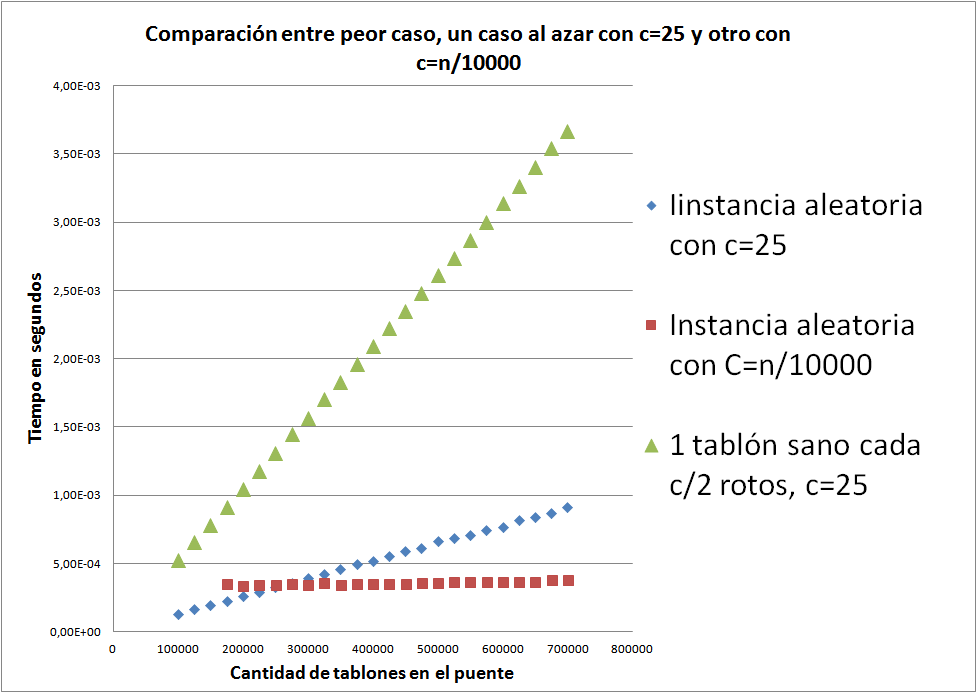
\includegraphics[scale=0.5]{ej1/graph_1.png}
\caption{Gráfico de tiempos para la ejecución de 3 instancias distintas. Peor caso e instancia aleatoria con c fijo y c dependiente de n}
\end{figure}

\begin{figure}[H]
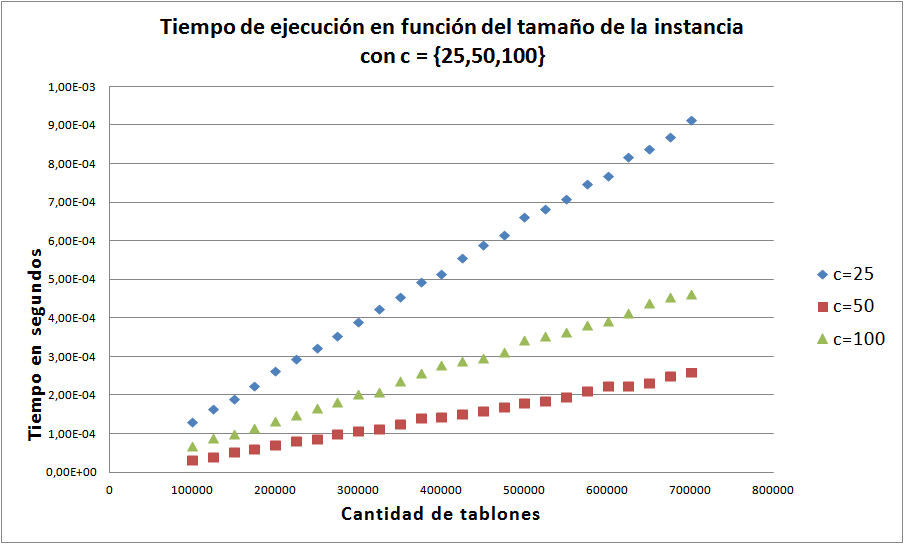
\includegraphics[scale=0.5]{ej1/graph_2.png}
\caption{Gráfico de tiempos para la ejecución de 3 instancias distintas. ($c=25$, $c=50$, $c=100$)}
\end{figure}

De la observación de los gráficos podemos notar el comportamiento lineal esperado de nuestro algoritmo para todas las instancias.

En el primer gráfico comprobamos empíricamente la existencia del peor caso que dedujimos de la demostración de complejidad. Este caso es considerablemente peor al de una instancia  aleatoria con el mismo c. A su vez notamos que, si el c respeta una misma proporción con el tamaño de la entrada, el algoritmo se comporta de forma más o menos constante ya que la cantidad de saltos presumiblemente será similar en todas las instancias (a lo sumo se modificará en 1 salto).
 
En el segundo gráfico vemos el impacto del c en el tiempo de ejecución para las mismas instancias aleatorias. A medida que se le permite saltar más tablones por vez, el algoritmo ejecuta cada vez más rápido.

Finalmente vale aclarar que no observamos distintas formas de distribuir tablones a lo largo del puente porque lo que realmente es significativo es si el tablón más lejano después de cada salto está roto o no y cuántos rotos seguidos hay antes de ese, siendo justamente el peor caso en cual hay exactamente la mitad del salto máximo de tablones.

Podemos entonces decir que este algoritmo se ve afectado en su tiempo por la cantidad máxima de tablones permitidos por salto y por la distribución de los tablones sobre el puente


\subsection{Adicionales}

\textbf{XXXXXXXXXXXXXXXXXXXXXXXXXXXXXXXXXXXXXXXXXXXXXXXXXXXXXXX}
\clearpage
%\include{ej2}
\section{Problema 3 - Biohazard}
\index{Problema 3 - Biohazard}


\subsection{Descripción del problema a resolver}

El problema que trataremos en la presente sección consiste en ubicar en la menor cantidad de camiones posibles una serie de compuestos químicos para su traslado. Cada producto tiene un nivel de peligrosidad con cada uno de los otros. A su vez, los camiones toleran hasta un margen $M$ de peligrosidad acumulada\footnote{La suma de todas las peligrosidades de los productois en su interior tomadas de a pares} en su interior (los camiones son iguales entre si). 

Se nos pide entonces un algoritmo capaz de asociar cada producto a un camión de forma tal de emplear los menos camiones posibles respetando los niveles de tolerancia impuestos. 

Notemos que este problema siempre tiene solución ya que si cada producto se ubica en solitario el traslado será seguro.

Como requerimiento extra tendremos que emplear la técnica algorítmica conocida como \textit{Backtracking} que detallaremos brevemente más adelante.

Veamos algunas instancias de este problema para entender algunos detalles más:

\begin{figure}[H]
\centering
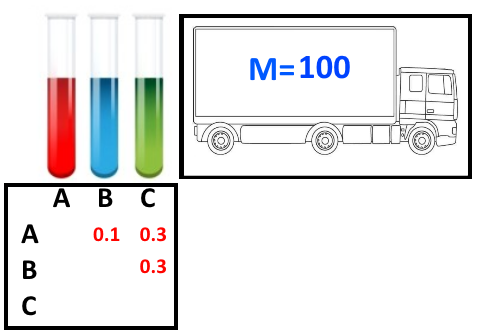
\includegraphics[scale=0.65]{ej3/instancia0.png}
\caption{Instancia con 3 productos y sus peligrosidades. Cada camión tolera hasta 100 de peligrosidad total}
\end{figure}


\begin{figure}[H]
\centering
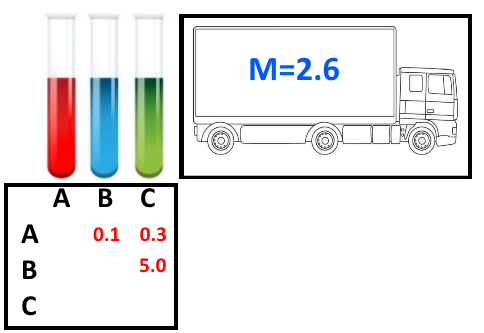
\includegraphics[scale=0.65]{ej3/instancia1.png}
\caption{Instancia con 3 productos y sus peligrosidades. Cada camión tolera hasta 2.6 de peligrosidad total}
\end{figure}

La representación de la entrada que recibiría el algoritmo para esta instancia se ve de la siguiente manera:

\begin{addmargin}[4em]{0em}
\textsf{8 3 0 0 1 1 1 1 0 0} \\
\textsf{0}
\end{addmargin}
\textbf{DESCRIPCIÓN DE LA ENTRADA}

Notemos que el producto A se lleva relativamente bien con el B y el C para los niveles tolerados por los camiones pero que B y C definitivamente no pueden compartir camión. Por este motivo la solución constará de 2 camiones en donde en un camión irá B, en otro C y A en cualquiera de ellos. 

Mientras la solución minimice los camiones, podremos devolver cualquiera de ellas. En particular nuestro algoritmo devuelve: 

\begin{addmargin}[4em]{0em}
\textsf{8 3 0 0 1 1 1 1 0 0} \\
\textsf{0}
\end{addmargin}

\textbf{DESCRIPCIÓN DE LA SALIDA}


\begin{figure}[H]
\centering
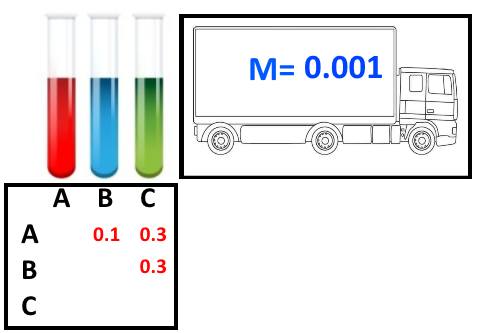
\includegraphics[scale=0.65]{ej3/instancia2.png}
\caption{Instancia con 3 productos y sus peligrosidades. Cada camión tolera hasta 0.0001 de peligrosidad total}
\end{figure}


%
%\subsection{Ideas desarrolladas para la resoluci\'on}
%Para el desarrollo de la resoluci\'on del problema nos basamos primeramente en el dibujo de la figura 1.1: pensamos que tenemos n productos, $p_{1} \dots p_ {n}$. Luego, cada producto $p_{i}$ hay que insertarlo en alg\'un cami\'on $c_{j}$. Como todos los camiones tienen el mismo l\'imite M de biohazard que soportan, es irrelevante en qu\'e n\'umero de cami\'on vamos a introducir cada producto. Lo \'unico que nos va a importar va a ser c\'omo distribuimos los productos de forma relativa entre ellos de tal forma que minimizemos la cantidad de camiones utilizados. Es decir, los camiones son indistinguibles entre s\'i. Con lo cual, como se puede ver en el dibujo, nuestro algoritmo en el paso $i$ prueba recursivamente con todas las combinaciones posibles que se pueden dar tras colocar el producto $p_{i}$ en alguno de los $k$ primeros camiones, donde $k$ es el \'indice del primer cami\'on que estaba  vac\'io antes del comienzo del paso i. Esta poda la nombramos en los comentarios del c\'odigo y la llamamos PODA 1.
%En el ejemplo, colocamos el producto 1 en el cami\'on 1, el 2 en el 1, el 3 en el 2 y el 4 en el 2. Con lo cu\'al, en el paso 5 vamos a probar todas las posibles combinaciones que pueden llegar a derivar de colocar el producto 5 en el cami\'on 1, 2 o 3. No tiene sentido probar qu\'e suceder\'ia colocando el producto 5 en el cami\'on 4 o 5 pues los camiones 3, 4 y 5 son indistinguibles con lo cual alcanza con elegir uno de estos. Nosotros optamos por elegir siempre el de menor \'indice. \\
%
%La otra poda importante que implementamos fue la de que cuando estamos buscando alg\'un cami\'on para colocar el producto $p_{i}$, nos fijamos si la cantidad de camiones ya utilizados en la subsoluci\'on actual (antes de agregar al producto $p_{i}$) es mayor que la mejor soluci\'on obtenida hasta el momento. Si este fuera el caso, entonces no analizamos los casos provenientes de agregar (para la configuraci\'on actual de productos en camiones) los productos $p_{i+1} \dots p_{n}$ porque ya sabemos que la soluci\'on que nos provean va a ser peor que la que ya conseguimos. Esta poda esta nombrada en el c\'odigo y la llamamos PODA 2. \\
%Observaci\'on: como la complejidad del algoritmo de por s\'i es muy grande, optamos por limitar la cantidad de productos que analizamos a 20, ya que para valores un poco m\'as grandes de $n$ sabemos que el algoritmo va a tardar mucho tiempo. \\
%
%\begin{center}
%    \includegraphics [width=20cm]{dibujo1_ej3.png}
%   {Fig. 3.1}
%\end{center}
%
%
%
%Para tener en cuenta, las estructuras de datos importantes de las que hacemos uso son:
%
%\begin{itemize}
%
%\item una matriz de enteros, hazards que dice para cada par de productos, cu\'al es el hazard que generan entre ellos
%\item un entero primerCamionVacio que lleva la cuenta de cu\'al es el \'indice del primer cami\'on vac\'io que en la soluci\'on temporal todav\'ia no usamos.
%\item un entero, mejorHastaAhora, que lleva la cuenta de la m\'inima cantidad de camiones que logramos utilizar para meter los productos hasta el momento
%\item un arreglo de enteros, resTemp, que lleva el resultados temporal (es decir, la data de en qu\'e cami\'on metimos cada uno de los productos considerados hasta el momento)
%\item un vector de enteros, productosEnCamion, que lleva la cuenta de qu\'e productos tenemos metidos en cada cami\'on.  
%\item un vector de enteros, hazardCamion, que lleva la cuenta para cada cami\'on, cu\'al es su hazard total en funci\'on de los productos que hay en \'el (siempre debe ser menor o igual a M)
%\item un arreglo de enteros, hazard2.En la posici\'on $i$ de este arreglo est\'a el hazard que genera el conjunto de productos representados por el entero $i$.
% 
%
%\end{itemize}
%
%
%A continuaci\'on vamos a introducir un pseudoc\'odigo con las ideas b\'asicas que tuvimos en cuenta a la hora de la implementaci\'on: \\
%
%resolver(producto i, resTemp): \\
%
% \hspace{1cm}if (me pase del ultimo producto) terminar \\
% 
% \hspace{2cm} for (camionj in 0 $\dots$ primer camion todav\'ia vac\'io): \\
%	\hspace{3cm} if (se puede agregar el producto i al camion camion camionj):\\
%    	\hspace{4cm} meter producto i en camion camionj, actualizando resTemp \\
%        \hspace{4cm} meter producto productoi en camion camionj \\
%        \hspace{4cm} actualizar el hazard del camion camionj \\
%        \hspace{4cm} if (camionj es el primer camion vacio): \\
%        	\hspace{5cm} actualizo primerCamionVacio \\
%            	
%        \hspace{4cm} if(puede ser mejor soluci\'on): resolver(producto i+1, resTemp) \\
%        
%        \hspace{4cm} if (llegue al \'ultimo producto): \\
%        	\hspace{5cm} if (primerCamionVacio $\leq$ mejorHastaAhora): \\
%            	\hspace{6cm} actualizo mejorHastaAhora = primerCamionVacio \\
%                \hspace{6cm} resultado = resTemp \\
%        \hspace{4cm} saco el producto i del camion camionj \\
%        \hspace{4cm} reestablezco el hazard que le corresponde al camion camionj \\
%        \hspace{4cm} if (camionj era el primer cami\'on todav\'ia vac\'io): \\
%        	\hspace{5cm} actualizo primerCamionVacio \\
%
% \hspace{1cm} terminar \\
% 
%
%
%% ESTARIA BUENO HACER EXPERIMENTOS PODANDO/NO PODANDO PARA VER COMO CAMBIA LA COMPLEJIDAD, MIRANDO GRAFIQUITOS.%
%
%\subsection{Justificaci\'on de complejidad}
%Primero que nada, se ve f\'acilmente que la funci\'on llenarHazards tiene una complejidad temporal de $O(n^{2} 2^{n})$. De esta forma, cada vez que queramos acceder al hazard total de un conjunto de productos vanos a tener acceso en $O(1)$	y no en $O(n)$. Vamos a ver que esta complejidad, necesaria para precalcular resultados que utilizaremos durante el backtracking, es menor que la complejidad del backtracking en s\'i mismo. Esto quiere decir que, esos c\'aclulos previos van a mejorar la los tiempos de ejecuci\'on del algoritmo, por la ganancia en tiempo de acceso al hazard total de un conjunto de productos. \\
%Algo destacable es que con esta implementaci\'on, ganamos complejidad temporal, pero perdemos complejidad espacial(usamos mucho espacio para guardar los hazards generados por todos los posibles subconjuntos de productos).
%
%%OPCION 1
%Para calcular la complejidad temporal de peor caso de nuestro algoritmo de backtracking, vamos a analizar, en funci\'on del para\'ametro de entrada $n$, la cantidad de resultados y sub-resultados intermedios que recorremos para decidir cu\'al es el ordenamiento \'optimo para nuestro problema en cuesti\'on. Como se puede ver, si no hici\'eramos podas, se cumplir\'ia la recurrencia $T(i) = i*T(i-1)$, a partir de la cual sencillamente se puede concluir que $T(n) = O(n!) \in O(n^n)$, por la f\'ormula de Stirling. \\
%
%%OPCION 2
%Sin embargo, con las podas que introdujimos, la complejidad temporal del algoritmo es $3^{n}$ porque en total visitamos $\sum\limits_{i=1}^n {n \choose i}2^{i}$ estados distintos en nuestro algoritmo (la igualdad se deduce de forma directa a partir de la F\'ormula de Binomios de Newton). Es decir, repetimos la funci\'on resolver $n$ veces, y en cada repetici\'on $i$, nos fijamos por cada forma de seleccionar esos $i$ productos de los $n$ que tenemos a disposici\'on, qu\'e suceder\'ia para cada una de esas $2^{i}$ formas de seleccionar dichos $i$ productos. \\
%
%
%
%
%
%
%\newpage
%A continuaci\'on, introducimos la parte m\'as relevante del c\'odigo que implementamos para la resoluci\'on del problema.
%\begin{lstlisting}
%void resolver(int productoi, int &primerCamionVacio, int &mejorHastaAhora, vector<int> &resTemp, vector<int> &res, vector<int> &hazardCamion,
%			  vector<int> &productosEnCamion, int &M, int &n, int hazard2[]) {
%    if(productoi == n) { return; }
%    int primerCamionVacioTemp = primerCamionVacio;
%          for(int camionj=0; camionj<=primerCamionVacioTemp; camionj++) {                
%                pair<bool, int> sePuedeAgregar = nuevoHazard(productoi,camionj,productosEnCamion,M,hazard2);
%                int hazardViejo = hazardCamion[camionj];
%                if(sePuedeAgregar.first) {					
%                    resTemp[productoi] = camionj + 1;
%                    productosEnCamion[camionj] += (1<<productoi)
%                    hazardCamion[camionj] = sePuedeAgregar.second
%                    if(camionj == primerCamionVacioTemp) {
%							primerCamionVacio++; 
%					}					
%                    if(primerCamionVacio <= mejorHastaAhora) {
%						resolver(productoi+1, primerCamionVacio, mejorHastaAhora, resTemp, res, hazardCamion, productosEnCamion, M, n, hazard2);
%                    }
%                    if(productoi + 1 == n) {				
%						  if(primerCamionVacio <= mejorHastaAhora) {													
%								mejorHastaAhora = primerCamionVacio;
%								res = resTemp;
%						  }
%					}
%                    productosEnCamion[camionj] -= (1<<productoi	
%                    hazardCamion[camionj] = hazardViejo;
%					if(camionj == primerCamionVacioTemp) { primerCamionVacio--; }		
%                } 
%          }
%          return;
%}
%\end{lstlisting}
% 
% 
%\subsection{Testeos de complejidad}
% 
% 
%En esta secci\'on, analizamos la i) complejidad del algoritmo sin podas, ii) complejidad del algoritmo con PODA 1, iii) complejidad del algoritmo con PODA 2, iv) complejidad del algoritmo con ambas podas. En el caso en que utilizamos las dos podas, estudiamos qu\'e sucede en los casos peor, promedio y mejor. \\ 
% 
% 
%\subsection{Análisis experimental de podas}
%
%


\newpage



\end{document}
